

\section{principle: least privilege}

\begin{frame}{least privilege}
    \begin{itemize}
    \item a typical program I run on my desktop is allowed to\ldots
    \item make network connections to anywhere
    \item upload all my files to the Internet
    \item delete all my files
    \item record all my keystrokes
    \item \ldots
    \vspace{.5cm}
    \item but it probably doesn't need to\ldots
    \item ideally: if typical program was compromised/malicious, \\
          it still wouldn't be able to do most of these things
    \end{itemize}
\end{frame}



\subsection{what do browsers need?}

\begin{frame}{things applications need?}
    \begin{itemize}
    \item what things should browser be able to do?
    \item what things should word processor be able to do?
    \end{itemize}
\end{frame}

\begin{frame}{things broswers need}
    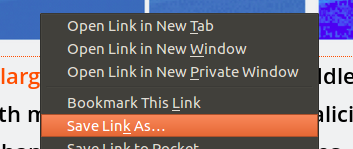
\includegraphics[width=.5\textwidth]{../sandbox/savelinkas}
    \begin{itemize}
        \item save files
        \item have your webmail password
        \item \ldots
    \end{itemize}
\end{frame}


\subsection{OS users}

\begin{frame}<1>[fragile,label=multiOS]{multi-user OSs}
\lstset{
    language={},style=small,
    moredelim={**[is][\color{red!70!black}]{~in~}{~end~}},
}
\begin{lstlisting}
cr4bd@labunix01:~$ ~in~cp myprogram.exe /bin/ls~end~
cp: cannot create regular file ‘/bin/ls’: Permission denied
\end{lstlisting}
    \begin{itemize}
        \item programs have \myemph{limited privileges}
        \item<2-> OS tracks ``user'' of running every program
        \item<2-> result: malware I installed shouldn't be able to effect other users
        \item<2-> idea 1: reuse this support for web browsers
            \begin{itemize}
            \item webpage should run as ``different user''
            \item malware should only affect web browser?
            \end{itemize}
    \end{itemize}
\end{frame}

\begin{frame}[fragile,label=permEnforce]{permission enforcement}
    \begin{minted}[fontsize=\small]{C}
struct Process {
    int user_id;
    ...
};
int handle_open_system_call(char *filename, ...) {
    Process* currentProcess = GetCurrentProcess();
    File* file = GetFileByFilename(filename);
    if (!file->UserCanAccess(currentProcess->user_id)) {
        return ERROR_PERMISSION_DENIED;
    }
    ...
}
\end{minted}
\end{frame}

\againframe<2>{multiOS}



\subsection{promise: privilege separation}

\begin{frame}{the privilege separation idea}
    \begin{itemize}
    \item can't make whole browser run as ``different user''
        \begin{itemize}
        \item still need to save files, read password, etc.
        \end{itemize}
    \item how about just the parts that are ``dangerous''?
        \begin{itemize}
        \item part that runs scripts, parses HTML
        \end{itemize}
    \end{itemize}
\end{frame}




\section{privilege separation: video decode}

\begin{frame}{simple privilege separation}
    \begin{itemize}
    \item simple example: want to show videos
    \item video decoding library is tens of thousands of lines of code
        \begin{itemize}
        \item often buggy, includes hard-to-check hand-written assembly
        \end{itemize}
    \item what does video decoding library do?
        \begin{itemize}
        \item read video file as input
        \item output images as output
        \end{itemize}
    \end{itemize}
\end{frame}

\begin{frame}{simple privilege seperation}
    \begin{itemize}
    \item setup: create new user
    \item start video decoder as new user
    \item communicate via ``pipes''
        \begin{itemize}
        \item like terminal to be used by program
        \end{itemize}
    \end{itemize}
\end{frame}

\begin{frame}[fragile,label=privSepOutline]{simple privilege seperation}
\begin{minted}[fontsize=\fontsize{10}{10}]{C}
/* dangerous video decoder to isolate */
int main() {
    /* switch to right user */
    SetUserTo("user-without-privileges"));
    while (fread(videoData, sizeof(videoData), 1, stdin) > 0) {
        doDangerousVideoDecoding(videoData, imageData);
        fwrite(imageData, sizeof(imageData), 1, stdout);
    }
}

/* code that uses it */
    FILE *fh = RunProgramAndGetFileHandle("./video-decoder");
    for (;;) {
        fwrite(getNextVideoData(), SIZE, 1, fh);
        fread(image, sizeof(image), 1, fh);
        displayImage(image);
    }
\end{minted}
\end{frame}




\subsection{another user is not enough}

\begin{frame}{issues with privilege separation (1)}
    \begin{itemize}
    \item ``other user'' can still do too much
    \vspace{.5cm}
    \item read unprotected files
        \begin{itemize}
        \item most of them?
        \end{itemize}
    \item write temporary files?
    \item open network connections
    \item use all your memory
    \item \ldots
    \end{itemize}
\end{frame}




\subsection{awkwardness of creating a new user}

\begin{frame}{issues with privilege separation (2)}
    \begin{itemize}
    \item awkward to do
    \item switching users requires special permissions
    \item seperate user for \myemph{each} video decoder, audio decoder, web page renderer?
        \begin{itemize}
        \item users can debug processes from same user
        \end{itemize}
    \item slowdown --- extra copying
    \end{itemize}
\end{frame}



\section{system calls as OS interface}
\begin{frame}{program to OS interface}
    \begin{itemize}
    \item primary way application talks to OS: system calls
    \vspace{.5cm}
    \item function calls that request OS do something
    \item typically: how program can interact with rest of system
        \begin{itemize}
        \item files
        \item other programs
        \item the network
        \item devices
        \item\ldots
        \end{itemize}
    \vspace{.5cm}
    \item controlling program behavior: control what system calls
    \end{itemize}
\end{frame}


\section{definition: sandbox}
\begin{frame}{``sandboxing''}
    \begin{itemize}
    \item result of filtering operations called a ``sandbox''
    \item idea: attacker can play in sandbox as much as they want
    \item can't do anything ``harmful''
    \vspace{.5cm}
    \item other possible implementations:
        \begin{itemize}
        \item e.g. virtual machine
        \end{itemize}
    \end{itemize}
\end{frame}




\section{Linux system call filtering}
\subsection{simple Linux system call filtering}
\newmintinline{C}{}
\begin{frame}{Linux system call filtering API}
    \begin{itemize}
    \item privilege seperation support: system call filtering
    \item simple API: \Cinline|seccomp(SECCOMP_SET_MODE_STRICT, 0, 0)|
        \vspace{.5cm}
            \item ``The only system calls the calling thread is permitted to make are \texttt{read},
                \texttt{write}, \texttt{\_exit}, and \texttt{sigreturn}. Other system calls [kill
                the program].''
            \item read/write only work on \myemph{already open files}
    \vspace{.5cm}
    \item later: what if we want to be finer-grained?
    \end{itemize}
\end{frame}


\section{aside: strace}
\begin{frame}[fragile]{strace hello\_world (1)}
\begin{lstlisting}[language=C,style=small]
#include <stdio.h>
int main() { puts("Hello, World!"); }
\end{lstlisting}
\hrule
when statically linked:
\begin{Verbatim}[fontsize=\fontsize{10}{11}\selectfont]
execve("./hello_world", ["./hello_world"], 0x7ffeb4127f70 /* 28 vars */)
                                        = 0
brk(NULL)                               = 0x22f8000
brk(0x22f91c0)                          = 0x22f91c0
arch_prctl(ARCH_SET_FS, 0x22f8880)      = 0
uname({sysname="Linux", nodename="reiss-t3620", ...}) = 0
readlink("/proc/self/exe", "/u/cr4bd/spring2023/cs3130/slide"..., 4096)
                                        = 57
brk(0x231a1c0)                          = 0x231a1c0
brk(0x231b000)                          = 0x231b000
access("/etc/ld.so.nohwcap", F_OK)      = -1 ENOENT (No such file or
                                                     directory)
fstat(1, {st_mode=S_IFCHR|0620, st_rdev=makedev(136, 4), ...}) = 0
write(1, "Hello, World!\n", 14)         = 14
exit_group(0)                           = ?
+++ exited with 0 +++
\end{Verbatim}
\end{frame}

\begin{frame}{aside: what are those syscalls?}
\begin{itemize}
\item execve: run program
\item brk: allocate heap space
\item arch\_prctl(ARCH\_SET\_FS, ...): thread local storage pointer
    \begin{itemize}
    \item may make more sense when we cover concurrency/parallelism later
    \end{itemize}
\item uname: get system information
\item readlink of /proc/self/exe: get name of this program
\item access: can we access this file [in this case, a config file]?
\item fstat: get information about open file
\item exit\_group: variant of exit
\end{itemize}
\end{frame}

\begin{frame}[fragile]{only after starting? (1)}
\begin{itemize}
\item okay, but that's only after starting up, right\ldots?
\item surely simpler if we limit system calls after startup
\item yes, but\ldots
\end{itemize}
\end{frame}

\begin{frame}[fragile]{only after starting? (2)}
\begin{lstlisting}[language=C,style=smaller]
#include <stdio.h>
int main() {
    FILE *fh = fopen("output.txt", "w");
    fprintf(fh, "example");
    fclose(fh);
}
\end{lstlisting}
\hrulefill
\begin{Verbatim}[fontsize=\fontsize{9}{10}]
$ strace ...
... [startup stuff, not shown] ...
openat(AT_FDCWD, "output.txt", O_WRONLY|O_CREAT|O_TRUNC, 0666) = 3
newfstatat(3, "", {st_mode=S_IFREG|0664, st_size=0, ...}, AT_EMPTY_PATH) = 0
write(3, "example", 7)                  = 7
close(3)                                = 0
\end{Verbatim}
\end{frame}

\begin{frame}[fragile]{only after starting? (2)}
\begin{lstlisting}[language=C,style=script]
#include <curl/curl.h>
int main() {
    CURL *handle = curl_easy_init();
    curl_easy_setopt(handle, CURLOPT_URL, "https://www.cs.virginia.edu/~cr4bd/test.txt");
    curl_easy_perform(handle);
    ...
}
\end{lstlisting}
\vspace{-.5cm}
\hrulefill
\begin{Verbatim}[fontsize=\fontsize{8}{9}]
$ strace ...
... [startup stuff, not shown] ...
futex(0x73f0bd640ba4, FUTEX_WAKE_PRIVATE, 2147483647) = 0                                               
...
openat(AT_FDCWD, "/usr/lib/ssl/openssl.cnf", O_RDONLY) = 3
...
sysinfo({...}) = 0
...
socket(AF_INET6, SOCK_DGRAM, IPPROTO_IP) = 3
close(3)                                = 0                                                             
socketpair(AF_UNIX, SOCK_STREAM, 0, [3, 4]) = 0                                                         
fcntl(3, F_GETFL)                       = 0x2 (flags O_RDWR)                                            
fcntl(3, F_SETFL, O_RDWR|O_NONBLOCK)    = 0                                                             
...
rt_sigaction(SIGPIPE, NULL, {sa_handler=SIG_DFL, sa_mask=[], sa_flags=0}, 8) = 0                        
...
socket(AF_INET, SOCK_STREAM, IPPROTO_TCP) = 5
setsockopt(5, SOL_TCP, TCP_NODELAY, [1], 4) = 0
...
getrandom("\xd6\x8c\xc3\x42\x07\x92"..., 48, 0) = 48 
...
\end{Verbatim}
\end{frame}



\subsection{more fine-grained filtering?}
\begin{frame}{Linux system call filtering: detailed}
    \begin{itemize}
    \item Linux supports more fine-grained system call filtering
    \item using BPF (Berkeley Packet Filter) programming language
        \begin{itemize}
        \item compiled in the kernel to assembly to check system calls
        \end{itemize}
    \vspace{.5cm}
    \item can check system call argument values, but\ldots
        \begin{itemize}
        \item problems with pointer arguments
        \item too many system calls
        \end{itemize}
    \end{itemize}
\end{frame}

\begin{frame}[fragile,label=open]{Linux system call: open}
\begin{lstlisting}[language=C,style=small]
open("foo.txt", O_RDONLY);
\end{lstlisting}
\begin{itemize}
\item parameters:
    \begin{itemize}
    \item system call number: 2 (``open'')
    \item argument 1: 0x7fffe983 (address of string ``foo.txt'')
    \item argument 2: 0 (value of ``\texttt{O\_RDONLY}'')
    \end{itemize}
\item very problematic to filter using BPF interface
\vspace{.5cm}
\item can deal with using `ptrace' --- Linux debugging interface
    \begin{itemize}
    \item BPF can trigger something like a debugger breakpoint
    \item breakpoint wakes up monitor program (attached like debugger)
    \item `monitor' program can perform system call on program's behalf
    \end{itemize}
\end{itemize}
\end{frame}

\begin{comment}
\begin{frame}[fragile,label=openRuleP1]{lots of ways to open (1)}
\begin{itemize}
\item let's say we want to disallow:
\end{itemize}
\begin{lstlisting}[language=C,style=smaller]
open("/dev/keyboard", O_RDONLY);
\end{lstlisting}
\begin{itemize}
\item problem 1: some other ways of doing that?
\begin{lstlisting}[language=C,style=smaller]
chdir("/dev");
open("keyboard, O_RDONLY);

open("../../../../../../dev/keyboard", O_RDONLY);

symlink("/dev", "/tmp/foo");
open("/tmp/foo/keyboard", O_RDONLY);
\end{lstlisting}
\end{frame}

\begin{frame}[fragile,label=openRuleP2]{lots of ways to open (2)}
\begin{itemize}
\item let's say we want to disallow:
\end{itemize}
\begin{lstlisting}[language=C,style=smaller]
open("/dev/keyboard", O_RDONLY);
\end{lstlisting}
\begin{itemize}
\item problem 2: filter language doesn't allow reading pointers
    \begin{itemize}
    \item string is passed via pointer
    \end{itemize}
\item problem 3: string can be changed from another core
    \begin{itemize}
    \item between when filter runs and when syscall runs
    \end{itemize}
\end{itemize}
\end{frame}

\begin{frame}[fragile,label=openRuleP3]{lots of ways to open (3)}
\begin{itemize}
\item let's say we want to disallow:
\end{itemize}
\begin{lstlisting}[language=C,style=smaller]
open("/dev/keyboard", O_RDONLY);
\end{lstlisting}
\begin{itemize}
\item problem 4: several other syscalls (that might be used innocently)
    \begin{itemize}
    \item openat, open\_by\_handle\_at
    \item would need to write additional filter rules
    \item \ldots or break programs that aren't trying to violate rule
    \end{itemize}
\end{itemize}
\end{frame}

\begin{frame}[fragile,label=howManySystemCalls]{Linux system calls}
\begin{itemize}
\item x86-64 linux: \myemph{313 system calls}
\item opening a file:
    \begin{itemize}
    \item open (number 2)
    \item openat (number 257)
    \item open\_by\_handle\_at (number 304)
    \end{itemize}
\item coordinating between threads (for using multiple cores):
    \begin{itemize}
    \item rt\_sigaction (number 13)
    \item rt\_sigprocmask (number 14)
    \item rt\_sigreturn (number 15)
    \item tkill (number 200)
    \item futex (number 202)
    \item set\_robust\_list (number 273)
    \item get\_robust\_list (number 274)
    \item more?
    \end{itemize}
\end{itemize}
\end{frame}
\end{comment}


\begin{frame}[fragile]{BPF filter example (1)}
\begin{itemize}
\item showing syntax for producing machine code from C macros / non-extended BPF
\end{itemize}
\begin{Verbatim}[fontsize=\fontsize{10}{11}]
// memory[offset of "nr"] --> accumulator
BPF_STMT(BPF_LD | BPF_W | BPF_ABS, (offsetof(struct seccomp_data, nr))),
// if (accumulator == SYS_write) PC += 1
BPF_STMT(BPF_JMP | BPF_JEQ, BPF_K, SYS_write, 1, 0),
// return "kill process"
BPF_STMT(BPF_RET | BPF_K, SECCOMP_RET_KILL_PROCESS),
// return "allow"
BPF_STMT(BPF_RET | BPF_K, SECCOMP_RET_ALLOW),
\end{Verbatim}
\end{frame}

\begin{frame}[fragile]{BPF filter example (2)}
\begin{Verbatim}[fontsize=\fontsize{10}{11}]
// memory[offset of "nr"] --> accumulator
BPF_STMT(BPF_LD | BPF_W | BPF_ABS, (offsetof(struct seccomp_data, nr))),
// if (accumulator == SYS_write) PC += 1 else PC += 0
BPF_STMT(BPF_JMP | BPF_JEQ, BPF_K, SYS_write, 1, 0),
// return "kill process"
BPF_STMT(BPF_RET | BPF_K, SECCOMP_RET_KILL_PROCESS),
// memory[offset of args[0]] --> accumulator
BPF_STMT(BPF_LD | BPF_W | BPF_ABS, (offsetof(struct seccomp_data, args[0]))),
// if (accumulator == 2) PC += 1 else PC += 0
BPF_STMT(BPF_JMP | BPF_JEQ, BPF_K, 2, 1, 0),
BPF_STMT(BPF_RET | BPF_K, SECCOMP_RET_KILL_PROCESS),
BPF_STMT(BPF_RET | BPF_K, SECCOMP_RET_ALLOW),
\end{Verbatim}
\end{frame}

\begin{frame}{other BPF operations}
    \begin{itemize}
    \item arithmetic (add, or, xor, \ldots)
    \item in eBPF (extended BPF): 10 additional registers
        \begin{itemize}
        \item not just accumulator
        \end{itemize}
    \end{itemize}
\end{frame}

\begin{frame}{running BPF fast/safely}
    \begin{itemize}
    \item idea: can verify in advance that\ldots
    \item there are no loops
    \item there are no out-of-bounds accesses
    \vspace{.5cm}
    \item convert to assembly function to run very fast
    \end{itemize}
\end{frame}


\subsection{aside: libseccomp}
\begin{frame}[fragile]{libseccomp}
    \begin{itemize}
    \item wrapper for writing BPF programs
    \item specify list of rules re: system call identifiers/arguments
    \item it generates BPF program with LDs, JMPs, etc.
    \end{itemize}
\begin{Verbatim}[fontsize=\small]
#define CHECK(x) if (!(x)) handle_error();
...
scmp_filter_ctx filter = seccomp_init(SCMP_ACT_KILL_PROCESS);
CHECK(seccomp_rule_add(filter, SCMP_ACT_ALLOW, SCMP_SYS(read), 0) == 0);
CHECK(seccomp_rule_add(filter, SCMP_ACT_ALLOW, SCMP_SYS(write), 0) == 0);
CHECK(seccomp_load(filter) == 0);
\end{Verbatim}
\end{frame}


\subsection{problems with filter}

\begin{frame}[fragile,label=openRuleP1]{lots of ways to open (1)}
\begin{itemize}
\item let's say we want to allow/disallow (but not `normal' files):
\end{itemize}
\begin{lstlisting}[language=C,style=smaller]
open("/dev/keyboard", O_RDONLY);
\end{lstlisting}
\begin{itemize}
\item problem 1: some other ways of doing that?
\end{itemize}
\begin{lstlisting}[language=C,style=smaller]
chdir("/dev");
open("keyboard", O_RDONLY);

open("../../../../../../dev/keyboard", O_RDONLY);

symlink("/dev", "/tmp/foo");
open("/tmp/foo/keyboard", O_RDONLY);
\end{lstlisting}
\end{frame}

\begin{frame}[fragile,label=openRuleP2]{lots of ways to open (2)}
\begin{itemize}
\item let's say we want to allow/disallow:
\end{itemize}
\begin{lstlisting}[language=C,style=smaller]
open("/dev/keyboard", O_RDONLY);
\end{lstlisting}
\begin{itemize}
\item problem 2: filter language doesn't allow reading pointers
    \begin{itemize}
    \item string is passed via pointer
    \end{itemize}
\item problem 3: string can be changed from another core
    \begin{itemize}
    \item between when filter runs and when syscall runs
    \end{itemize}
\end{itemize}
\end{frame}

\begin{frame}[fragile,label=openRuleP3]{lots of ways to open (3)}
\begin{itemize}
\item let's say we want to disallow:
\end{itemize}
\begin{lstlisting}[language=C,style=smaller]
open("/dev/keyboard", O_RDONLY);
\end{lstlisting}
\begin{itemize}
\item problem 4: several other syscalls (that might be used innocently)
    \begin{itemize}
    \item openat, open\_by\_handle\_at
    \item would need to write additional filter rules
    \item \ldots or break programs that aren't trying to violate rule
    \end{itemize}
\end{itemize}
\end{frame}

\begin{frame}[fragile,label=howManySystemCalls]{Linux system calls}
\begin{itemize}
\item x86-64 linux: \myemph{313 system calls}
\item opening a file:
    \begin{itemize}
    \item open (number 2)
    \item openat (number 257)
    \item open\_by\_handle\_at (number 304)
    \end{itemize}
\item coordinating between threads (for using multiple cores):
    \begin{itemize}
    \item rt\_sigaction (number 13)
    \item rt\_sigprocmask (number 14)
    \item rt\_sigreturn (number 15)
    \item tkill (number 200)
    \item futex (number 202)
    \item set\_robust\_list (number 273)
    \item get\_robust\_list (number 274)
    \item more?
    \end{itemize}
\end{itemize}
\end{frame}


\subsection{shared services?}
\begin{frame}{shared services?}
    \begin{itemize}
    \item often programs do operations by talking to ``server'' program
        \begin{itemize}
        \item example: GUI management on Linux (X11 or Wayland), OS X (WindowServer)
        \item example: mixing sound from multiple applications
        \item \ldots
        \end{itemize}
    \item whole extra set of calls to sanitize
        \begin{itemize}
        \item when to allow ``get keyboard input'' for GUI
        \item when to allow ``get microphone input'' for sound manager
        \item making sure one isn't manipulating wrong program's windows?
        \end{itemize}
    \item also, server programs might have security problems
        \begin{itemize}
        \item common ``sandbox escape''
        \end{itemize}
    \end{itemize}
\end{frame}



\subsection{more sophisticated filters}
\section{Chrome architecture}
\usetikzlibrary{positioning,shapes.callouts}

\begin{frame}{Chrome architecture}
    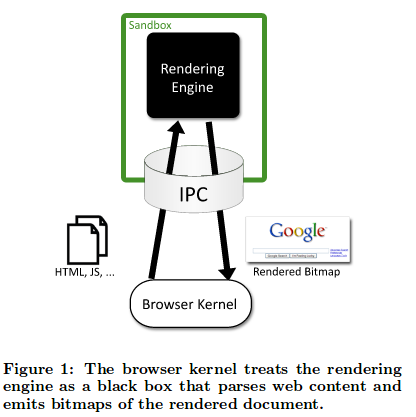
\includegraphics[height=0.8\textheight]{../sandbox/chrome-arch}
\end{frame}

\begin{frame}{talking to the sandbox}
    \begin{itemize}
    \item browser kernel sends commands to sandbox
    \item sandbox sends commands to browser kernel
    \item idea: commands only allow necessary things
    \end{itemize}
\end{frame}

\begin{frame}{original Chrome sandbox interface}
    \begin{itemize}
        \item sandbox to browser ``kernel''
            \begin{itemize}
                \item show this image on screen
                \begin{itemize}
                    \item (using shared memory for speed)
                \end{itemize}
            \item \myemph<2-3>{make request\tikzmark{request} for this URL}
            \item \myemph<4>{download\tikzmark{download} files to local FS}
            \item \myemph<5>{upload\tikzmark{upload} user requested files}
            \end{itemize}
        \item browser ``kernel'' to sandbox
            \begin{itemize}
                \item send user input
            \end{itemize}
    \end{itemize}
    \begin{tikzpicture}[overlay,remember picture]
        \coordinate (middle) at ([yshift=-1cm]current page.center);
        \begin{visibleenv}<2>
            \node[my callout=request,anchor=center,align=center]  at (middle) {
                needs filtering --- at least no \texttt{file:} (local file) URLs
            };
        \end{visibleenv}
        \begin{visibleenv}<3>
            \node[my callout=request,anchor=center,align=center] at (middle) {
                can still read any website! \\
                still sends normal cookies!
            };
        \end{visibleenv}
        \begin{visibleenv}<4>
            \node[my callout=download,anchor=center,align=center] at (middle) {
                files go to download directory only \\
                can't choose arbitrary filenames
            };
        \end{visibleenv}
        \begin{visibleenv}<5>
            \node[my callout=upload,anchor=center,align=center] at ([yshift=-1cm]middle) {
                browser kernel displays file choser \\
                only permits files selected by user
            };
        \end{visibleenv}
    \end{tikzpicture}
\end{frame}



% FIXME: Chrome Site Isolation
\subsection{Site Isolation}
% https://www.usenix.org/conference/usenixsecurity19/presentation/reis

\begin{frame}{Site Isolation}
\begin{itemize}
\item Chrome since version 67 (desktop)/77 (Mobile) has process per site
\item site $\approx$ registered domain name (example.com, example.co.uk, etc.)
    \begin{itemize}
    \item slightly different than same origin policy
    \end{itemize}
\vspace{.5cm}
\item complicated to implement:
    \begin{itemize}
    \item single web page can embed content from multiple other sites
        \begin{itemize}
        \item and those other sites can embed content from yet more sites
        \end{itemize}
    \item web page can call services on other websites with ``permission'' of other website
    \item clicking link may or may not requiring switching to new process
    \end{itemize}
\vspace{.5cm}
\item same separation being prototyped in recent Firefox builds
\end{itemize}
\end{frame}


\section{OpenSSH architecture}
\begin{frame}{OpenSSH privilege seperation}
    \begin{itemize}
    \item OpenSSH uses privilege seperation for its SSH server
    \item what runs on the lab machines when you log into them
    \vspace{.5cm}
    \item separate network processing code from authentication code
    \item seperate process per connection --- users don't share
    \vspace{.5cm}
    \item developed before system call filtering was widely available
        \begin{itemize}
        \item uses separate user + chroot (we'll talk later) to isolate
        \end{itemize}
    \end{itemize}
\end{frame}

\begin{frame}{OpenSSH privsep protocol}
    \begin{itemize}
    \item sandboxed process tells ``monitor'' to:
        \vspace{.25cm}
    \item perform \myemph{cryptographic operations}
        \begin{itemize}
        \item long-term keys never in sandboxed process
        \item commands to ask for cryptographic messages they need
        \end{itemize}
    \item ask to switch to user --- if given user password, etc.
        \begin{itemize}
            \item \myemph{monitor process verifies} login information
        \end{itemize}
    \item after authentication: new process running as logged-in user 
        \begin{itemize}
            \item (normally) no issues with special privileges
        \end{itemize}
    \end{itemize}
\end{frame}


\begin{frame}{privilege seperation overall}
    \begin{itemize}
    \item large application changes
        \begin{itemize}
        \item OpenSSH: 3k lines of code for communication/etc. added
        \item OpenSSH: 2\% of existing code (950 of 44k lines) changed
        \item (but most changes simple)
        \end{itemize}
    \item lots of application knowledge
        \begin{itemize}
        \item what is a meaningful separation of `privileged' and `unprivileged'?
        \end{itemize}
    \item better application design anyways?
    \end{itemize}
\end{frame}



\subsection{exercise: priv sep for}
\begin{frame}{privilege separation for}
    \begin{itemize}
    \item let's say we wanted to add sandboxing/privilege separation to an (standalone) mail program
    \vspace{.5cm}
    \item exercise 1: where would be concerned about security problems?
    \item exercise 2: propose a way of dividing up the program
    \end{itemize}
\end{frame}



\subsection{versus capability-type approach}
\begin{frame}{changing what programs can name}
    \begin{itemize}
    \item seccomp, separate users: program tries to access X, checks if allowed
    \vspace{.5cm}
    \item alternate idea: changing what Xs program can name
    \end{itemize}
\end{frame}

\begin{frame}{aside: capabilities/ambient authority (1)}
    \begin{itemize}
    \item user permissions --- authority tied to each running program
    \item ``access control lists'' for resources
    \item sometimes called ``ambient authority''
    \vspace{.5cm}
    \item alternate model: ``capabilities''
    \item running program has list of things it can access/how
    \end{itemize}
\end{frame}

\begin{frame}{aside: capabilities/ambient authority (2)}
    \begin{itemize}
    \item capabilities = program has list of things it can access
    \item most common thing with design: open files
    \vspace{.5cm}
    \item used as basis of some operating system designs
        \begin{itemize}
        \item not desktop OSes, but\ldots
        \item Unix/Linux has many things with `flavor' of capabilities
        \end{itemize}
    \item in ``fully'' capability-based OSes also\ldots
        \begin{itemize}
        \item capabilities for accessing non-regular-file resources (processes, directories,
            network ports, \ldots)
        \item way of transferring capabilities between programs (instead of, e.g., filenames/PIDs/etc.)
        \item OS doesn't track user IDs/etc. (though maybe system services do)
        \end{itemize}
    \end{itemize}
\end{frame}


\subsection{chroot}
\begin{frame}{Unix filesystems and mounting}
    \begin{itemize}
    \item my Linux desktop has two disks:
        \begin{itemize}
        \item \texttt{/} --- an SSD
        \item \texttt{/mnt/extradisk} --- a hard drive
        \end{itemize}
    \item hard drive appears as \textit{subdirectory} of SSD
    \item subdirectory called a \textit{mount point}
    \end{itemize}
\end{frame}

\begin{frame}[fragile,label=perProcessRoot]{per-process root}
    \begin{itemize}
    \item on Unix: each process tracks its own root directory (/)
    \item can be changed with chroot() system call
        \begin{itemize}
        \item command-line tool to access: \texttt{chroot}
        \end{itemize}
    \vspace{.5cm}
    \item usage: can isolate program from other files on system
        \begin{itemize}
        \item example: limit what public file server can access?
        \end{itemize}
    \end{itemize}
\end{frame}

\begin{frame}[fragile,label=lsChrootExample]{chroot ls}
\begin{lstlisting}[language={},style=smaller]
# mkdir /tmp/example
# cp /bin/ls /tmp/example/ls
# chroot /tmp/example /ls
chroot: failed to run command ‘/ls’: No such file or directory
# cp -r /lib64 /tmp/example/lib64
# mkdir -p /tmp/example/lib
# cp -r /lib/x86_64-linux-gnu /tmp/example/lib/x86_64-linux-gnu
# chroot /tmp/example /ls
/ls: error while loading shared libraries: libpcre2-8.so.0: cannot open shared object file: No such file or directory
# cp /usr/lib/x86_64-linux-gnu/libpcre2-8* /tmp/example/lib/x86_64-linux-gnu
# chroot /tmp/example /ls /
lib  lib64  ls
# chroot /tmp/example /ls /..
lib  lib64  ls
# 
\end{lstlisting}
\end{frame}

\begin{frame}{chroot escapes}
    \begin{itemize}
    \item chroot prevents accessing files outside the new \texttt{/}
    \item but root (system adminstrator) user in chroot can access disks, etc.
    \vspace{.5cm}
    \item typical usage: combine chroot with extra user
    \end{itemize}
\end{frame}

\begin{frame}{chroot impracticality}
    \begin{itemize}
    \item some things make chroot impractical in general:
    \vspace{.5cm}
    \item seems like one needs extra copies of most of the system
    \item hard to communicate between separate roots
    \item requires administrator permissions to configure
        \begin{itemize}
        \item dangerous to let normal users configure b/c they could confuse priviliged (set-user-ID) programs like \texttt{sudo}
        \end{itemize}
    \end{itemize}
\end{frame}


\subsubsection{exercise}
\begin{frame}{exercise}
    \begin{itemize}
    \item what scenarios does chroot make most/least sense for?
    \begin{itemize}
        \item A. the rendering part of web browser
        \item B. a web server
        \item C. a media player
        \item D. a network time server (for other machines to set their clocks)
    \end{itemize}
    \end{itemize}
\end{frame}


\subsection{Linux namespaces}
\begin{frame}{Linux namespaces (1)}
    \begin{itemize}
    \item Linux: alternate sandboxing features
    \item ``namespaces'' for other resources
    \item chroot: each process has own idea of root directory
        \begin{itemize}
        \item change to OS: look up root directory in process, not global variable
        \end{itemize}
    \item can apply this to other resources:
        \begin{itemize}
        \item what filesystems (disks) are available
        \item what network devices are available
        \item what user identifier numbers are
        \item \ldots
        \end{itemize}
    \end{itemize}
\end{frame}

\begin{frame}{Linux namespaces (2)}
    \begin{itemize}
    \item user namespace:
    \vspace{.5cm}
    \item can run programs with new view of users:
    \vspace{.5cm}
    \item inside namespace: running as root
    \item outside namespace: root translated to innocent user ID
    \item allows running programs that expect different users
        \begin{itemize}
        \item \ldots without changes, but without giving special permissions
        \end{itemize}
    \vspace{.5cm}
    \item mechanism: reassign user ID numbers in kernel
        \begin{itemize}
        \item figuring out what user ID means --- always apply current process mapping
        \end{itemize}
    \end{itemize}
\end{frame}

\begin{frame}[fragile,label=LinuxCloneUnshare]{aside: Linux clone(), unshare() syscalls}
\begin{itemize}
\item Linux clone system call: start new process (or thread)
\item flags to specify environment of new process
\item these flags can include ``make a new namespace of a type''
\end{itemize}
\begin{lstlisting}[style=smaller,language=C++]
int id = clone(start_function, ..., CLONE_NEWUSER | other-flags);
\end{lstlisting}
\begin{itemize}
\item above option: new user namespace for new process
\vspace{.5cm}
\item alternative: for changing current process's namespace:
\end{itemize}
\begin{lstlisting}[style=smaller,language=C++]
unshare(CLONE_NEWUSER);
\end{lstlisting}
\end{frame}

\begin{frame}{user namespaces API}
\begin{itemize}
\item Linux: users identified by numerical \textit{user IDs} (UIDs)
\vspace{.5cm}
\item with user namespaces:
\item control file \texttt{/proc/PROCESS-ID/UID\_MAP} contains lines like:
    \begin{itemize}
    \item \texttt{0 1000 2} --- UID 0--1 maps to UID 1000--1001
    \item \texttt{1000 2000 100} --- UID 1000-1100 maps to UID 2000--2100
    \end{itemize}
\item can write to that file to reconfigure (if enough permissions)
\end{itemize}
\end{frame}

\begin{frame}{Linux namesapces (3)}
    \begin{itemize}
    \item mount namespaces:
        \begin{itemize}
        \item Unix: mounting disk = making the contents of the disk available as directories+files
        \end{itemize}
    \vspace{.5cm}
    \item different idea of what filesystems are available
    \item can be setup with \textit{bind mounts} to ``real FS''
        \begin{itemize}
        \item but otherwise: no access to directories outside mount namespace
        \item normally requires root --- but special case with user namespaces
        \end{itemize}
    \end{itemize}
\end{frame}

\begin{frame}[fragile,label=mountNSCmdLine]{mount namespaces API}
from command line:
\begin{lstlisting}[language={},style=smaller]
    # runs shell (/bin/sh) in new mount namesapce
shell1$ unshare --mount /bin/sh

    # setup directories in /tmp/workdir and make them aliases of things on normal FS 
    # these aliases will only exist for processes in mount namespace
shell2$ mkdir -p /tmp/workdir/bin
shell2$ mkdir -p /tmp/workdir/lib
shell2$ mkdir -p /tmp/workdir/usr
shell2$ mkdir -p /tmp/workdir/current
shell2$ mount -o bind,ro /bin /tmp/workdir/bin
shell2$ mount -o bind,ro /lib /tmp/workdir/lib
shell2$ mount -o bind,ro /usr /tmp/workdir/usr
shell2$ mount -o bind /home/someuser /tmp/workdir/current

    # start new shell with the root directory being /tmp/workdir
shell2$ chroot /tmp/workdir /bin/sh
shell3$ cd /
shell3$ /bin/ls
bin     current     lib     usr
\end{lstlisting}
\end{frame}

\begin{frame}{Linux namespaces (3)}
    \begin{itemize}
    \item user namespace and mount namespace together:
    \vspace{.5cm}
    \item run program in new user namespace
    \item map regular root (in namespace) to regular user
        \begin{itemize}
        \item ``opts out'' of programs like sudo
        \end{itemize}
    \item move to new mount namespace
    \item setup bind mounts + chroot
        \begin{itemize}
        \item special case: allowed because root in user namespce
        \item can't get ``real'' root (administrator) privileges ever
        \end{itemize}
    \item run program with subset of available files
    \end{itemize}
\end{frame}

\begin{frame}{Linux namespaces (4)}
    \begin{itemize}
    \item other resources with namespaces
    \item network --- common usage: virtual network device for set processes
        \begin{itemize}
        \item different ``what is my IP address?'' answer for different processes
        \end{itemize}
    \item hostname (``UTS'')
    \item process identifiers
    \item control groups (resource limits for memory, CPU usage, disk I/O, etc.)
    \end{itemize}
\end{frame}

\begin{frame}{Linux control groups}
    \begin{itemize}
    \item control groups --- tied to namespaces
    \item primarily: CPU/memory/IO performance restrictions
        \begin{itemize}
        \item primarily intended for `friendly sharing' (containers, etc.)
        \item important for preventing denial-of-service/etc.
        \item not as big a security conern as file/user/etc. access
        \end{itemize}
    \item also mechanism for adding IO device restrictions
    \item also mechanism to start/stop a bunch of processes together
    \end{itemize}
\end{frame}


% FIXME: Chrome sandboxing failing:
    % https://theori.io/research/escaping-chrome-sandbox/
        % Binder (Chrome internal IPC library)
    % % https://googleprojectzero.blogspot.com/2020/04/you-wont-believe-what-this-one-line.html
    % https://bugs.chromium.org/p/project-zero/issues/detail?id=1991
    % https://bugs.chromium.org/p/project-zero/issues/detail?id=1985

% FIXME: SELinux sandbox escape:
    % https://www.openwall.com/lists/oss-security/2016/09/25/1

\subsection{Linux programs that attempt confinement}
\begin{frame}{Linux sandboxing programs, generally}
    \begin{itemize}
    \item docker, lxc, lxd, containerd
        \begin{itemize}
        \item use namespaces to create ``container'' with own copy of OS libraries, services
        \item but containers share OS `kernel' and potentially files with host unlike VM
        \item (might also have options to use other ways of getting this functionality --- VM's, etc.)
        \end{itemize}
    \item bubblewrap, firejail
        \begin{itemize}
        \item use Linux namespace tools + ``bind mounts'' to give programs only subset of files, etc.
        \item firejail has option of running a ``proxy'' windowing system server
        \end{itemize}
    \item SELinux's sandbox
        \begin{itemize}
        \item uses Security Enhanced Linux's mandatory access controls instead of Linux namespaces
        \item includes option for ``proxy'' for windoing system server
        \end{itemize}
    \end{itemize}
\end{frame}


\subsection{containers}
\begin{frame}{containers}
    \begin{itemize}
    \item Linux's seccomp + namespaces + SELinux commonly used to implement containers
        \begin{itemize}
        \item (plus cgroups (control groups) for performance isolation)
        \end{itemize}
    \vspace{.5cm}
    \item usual goal: looks like virtual machine, but much lower overhead
    \item examples: Docker, Kubernetes
        \begin{itemize}
        \item (note: these may also support other ways of creating `lightweight VMs')
        \end{itemize}
    \end{itemize}
\end{frame}




\begin{frame}{sandbox escapes generally}
    \begin{itemize}
    \item bug in sandbox interface
        \begin{itemize}
        \item example: memory/injection error in handling inputs
        \end{itemize}
    \item unintended functionality of sandboxed operations
    \end{itemize}
\end{frame}

\subsubsection{runC bug}
\begin{frame}{runc bug}
    \begin{itemize}
    \item 2019 bug in Docker, other container implementations (CVE-2019-5736)
        \begin{itemize}
        \item blog post for vulnerability finders: \\\scriptsize \url{https://blog.dragonsector.pl/2019/02/cve-2019-5736-escape-from-docker-and.html}
        \end{itemize}
    \vspace{.5cm}
    \item bug setup:
        \begin{itemize}
        \item user starts malicious container X
        \item user tells docker to start a new command in malicious container X
        \item \myemph<2>{malicious container X hijacks the ``new command'' starting program}
        \item hijacked program used to access stuff outside container
        \end{itemize}
    \item part of problem: Docker and others weren't using user namespaces at the time
        \begin{itemize}
        \item compatability problems
        \end{itemize}
    \end{itemize}
\end{frame}

\begin{frame}{setup: /proc/PID}
    \begin{itemize}
    \item Linux provides /proc directory to access info about programs
    \item used for implementing process list utils, debugging
        \begin{itemize}
        \item needed to make a functional container
        \end{itemize}
    \item subdirectory for each process in current container
        \begin{itemize}
        \item process ID PID has /proc/PID subdirectory
        \item /proc/self is alias for current process's subdirectory
        \end{itemize}
    \vspace{.5cm}
    \item included is /proc/PID/exe file --- alias for executable file
    \end{itemize}
\end{frame}

\begin{frame}{running a command in existing container}
    \begin{itemize}
    \item to run command X in existing container:
    \vspace{.5cm}
    \item step 1: switch current process to that container
    \item<2-> \myemph{code in container can access /proc here?}
    \item<2-> \myemph{including overwriting /proc/self/exe!}
        \begin{itemize}
        \item which is a program run as root!
        \end{itemize}
    \vspace{.25cm}
    \item step 2: execute command X
    \end{itemize}
\end{frame}


\begin{frame}{partial fix}
    \begin{itemize}
    \item can disable access to /proc/PID/exe (and related things)
    \item system call: \texttt{prctl(PR\_SET\_DUMPABLE, 0)}
    \item but\ldots the run-in-container tool did this for a while
    \vspace{.5cm}
    \item<2-> problem: this gets reset on executing a new program
    \item<2-> and attacker could make the new program be /proc/PID/exe
        \begin{itemize}
        \item one mechanism: symbolic links (file aliases)
        \end{itemize}
    \item<2-> but change dynamic linking setup to run attacker code
    \item<2-> \ldots which accesses /proc/self/exe
    \end{itemize}
\end{frame}

\begin{frame}{full fix}
    \begin{itemize}
    \item make single-use copy of start-in-container tool each time command run
        \begin{itemize}
        \item in-memory file
        \end{itemize}
    \item \ldots so modifying it doesn't change anything
        \begin{itemize}
        \item (but it's also protected from modification)
        \end{itemize}
    \vspace{.5cm}
    \item other solutions:
        \begin{itemize}
        \item make executable non-writable (e.g. SELinux, don't run container as root)
        \end{itemize}
    \end{itemize}
\end{frame}



\subsubsection{Chrome sandbox escapes}
\begin{frame}{Chrome sandbox escape (1)}
    \begin{itemize}
    \item recall: renderer communicates with `browser kernel'
    \item `browser kernel' might have bugs in this interface
        \begin{itemize}
        \item example: \url{https://project-zero.issues.chromium.org/issues/42451090} --- missing access check for `wrong' website
        \item example: \url{https://chromereleases.googleblog.com/2021/09/stable-channel-update-for-desktop.html} \url{https://starlabs.sg/blog/2022/01-the-cat-escaped-from-the-chrome-sandbox/} --- use after free in API available from renderer
        \end{itemize}
    \end{itemize}
\end{frame}

\begin{frame}{Chrome sandbox escape (2)}
    \begin{itemize}
    \item Chrome Windows sandbox
    \item based on ``restricted access tokens''
        \begin{itemize}
        \item on Windows, programs have `access tokens' representing their permissions
        \item can create `restricted' version to limit access
        \end{itemize}
    \end{itemize}
\end{frame}
\begin{frame}{Chrome sandbox escape (3)}
    \begin{itemize}
    \item {\tiny \url{https://googleprojectzero.blogspot.com/2020/04/you-wont-believe-what-this-one-line.html}}:
    \item problem: Windows erronously allowed starting new processes with a more unrestricted token
        \begin{itemize}
        \item supposed to have check where the token being used came from, but incomplete
        \end{itemize}
    \item \ldots but needed to get `handle' to that token
    \item solution: ask to duplicate another running process
    \end{itemize}
\end{frame}


\section{the Android sandbox}
\begin{frame}{Android sandbox}
    \begin{itemize}
    \item Android --- Linux based OS for phones/tablets
    \vspace{.5cm}
    \item \url{https://source.android.com/security/app-sandbox}
    \item current version: SELinux + seccomp (system call filter)
    \end{itemize}
\end{frame}


% FIXME: Android sandbox

\subsection{OSX sandboxing}

\begin{frame}{OS X sandboxing}
    \begin{itemize}
    \item OS X (tries to) implement system call filtering
    \item main challenge: what about files?
        \begin{itemize}
        \item user can open a file anywhere --- we expect that to work
        \end{itemize}
    \item<2> OS X solution: OS service displays file-open dialog
        \begin{itemize}
        \item OS knows user really choose a file
        \end{itemize}
    \item<2> application can ask to remember file was chosen previously
    \item<2> not chosen/remembered --- can't access
        \begin{itemize}
        \item requires changes to how applications open files
        \end{itemize}
    \end{itemize}
\end{frame}


\subsection{Qubes}

\begin{frame}{another sandboxing OS: Qubes}
    \begin{itemize}
    \item Qubes: heavily sandboxed OS
    \item runs \myemph{seperate VMs} instead of filtering syscalls
    \item UI that clearly shows what VM each window is from
    \vspace{.5cm}
    \item advantage: easier to gaurentee isolation
        \begin{itemize}
        \item many, many more bugs in system call filtering than VMs
        \end{itemize}
    \item disadvantage: harder to share between VMs
    \item disadvantage: much more runtime overhead
    \end{itemize}
\end{frame}

\begin{frame}{Qubes screenshot}
    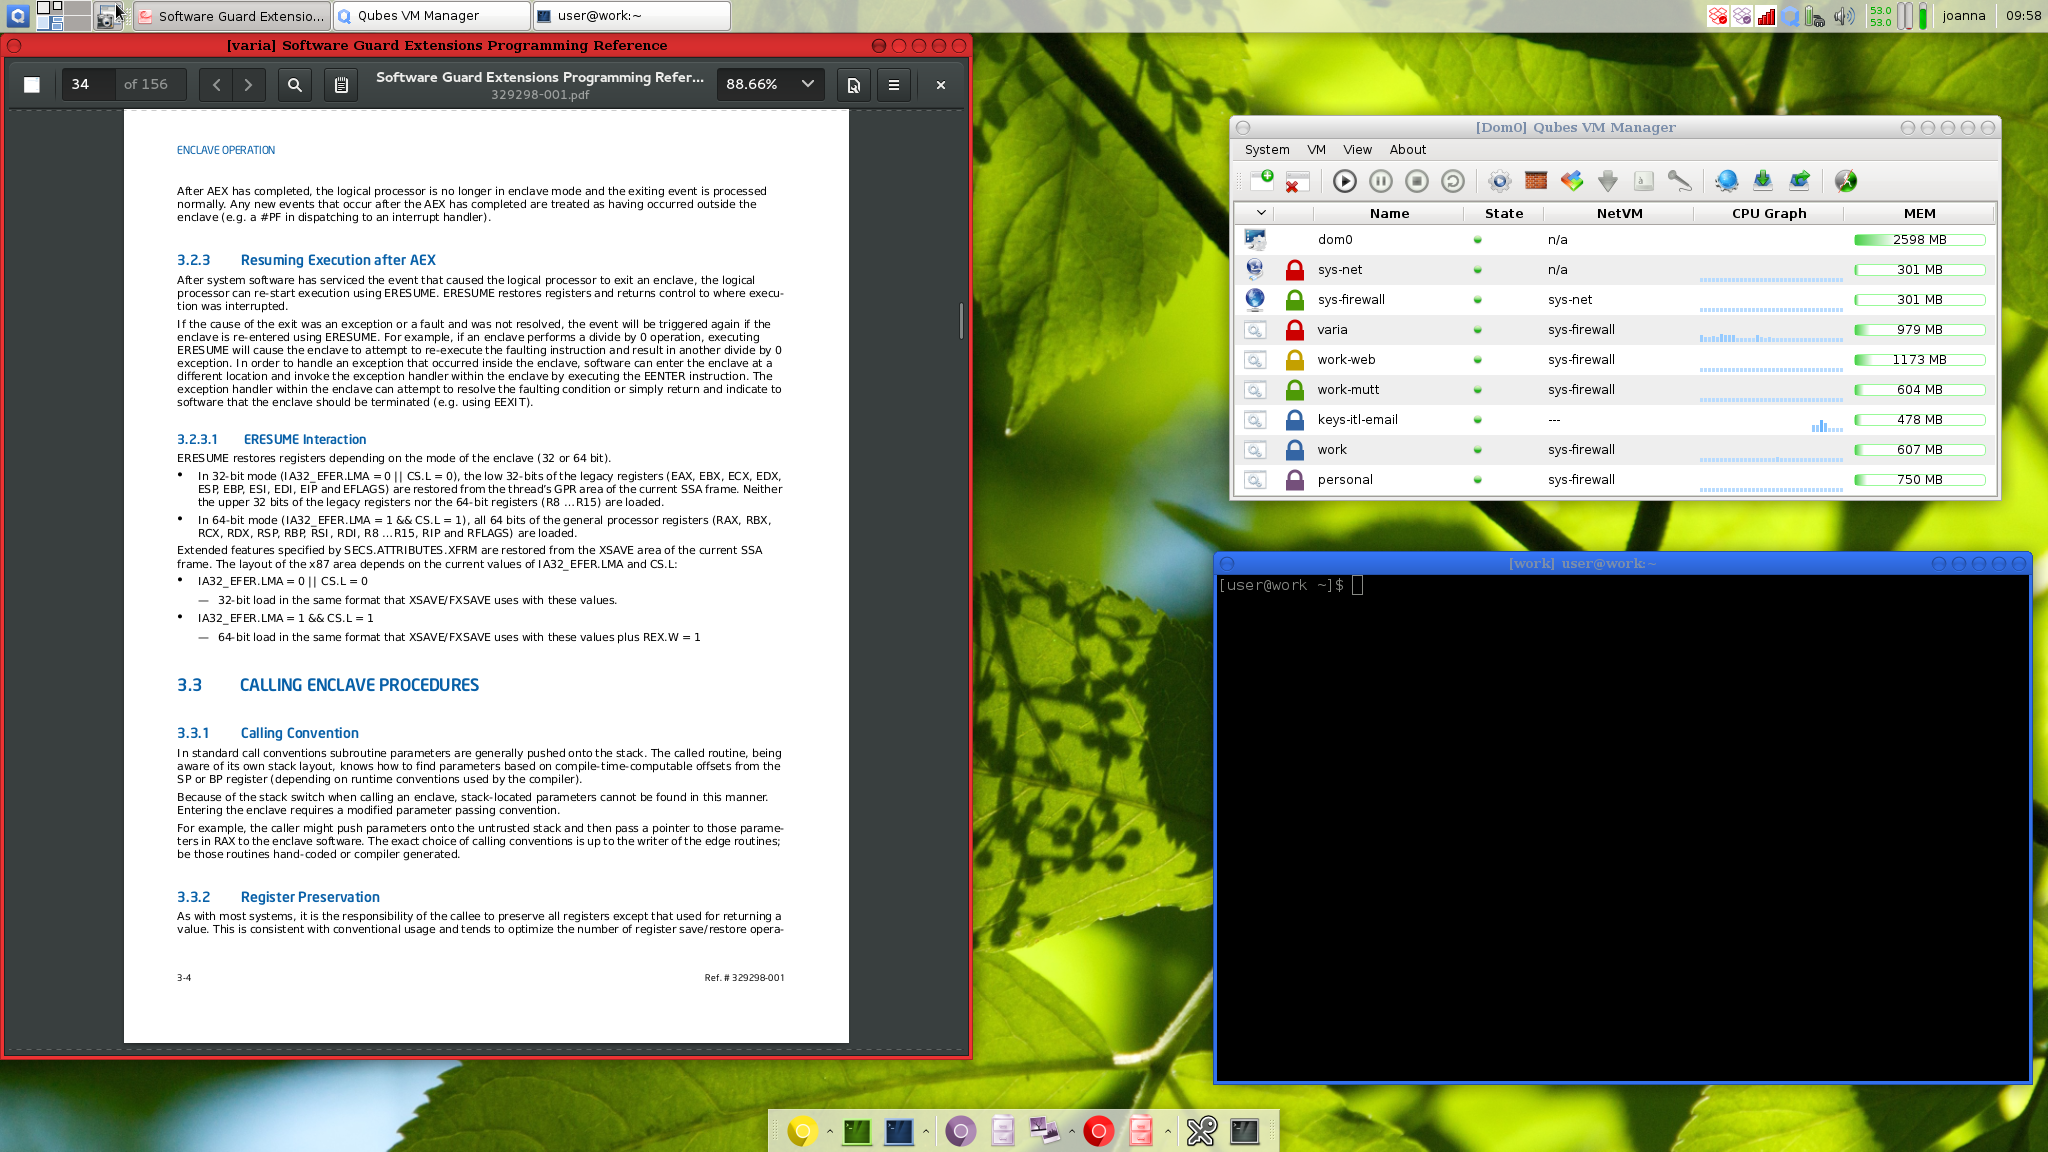
\includegraphics[width=\textwidth]{../sandbox/qubes-desktop1}
\end{frame}




\section{Which sandboxing?}
\begin{frame}{which sandboxing?}
    \begin{itemize}
    \item which whole-application sandboxing technique seems better for 
        \begin{itemize}
        \item security, performance, usability, handling unchanged applications
        \end{itemize}
    \item (full answer: could mix techniques + probably depends on details of app)
    \vspace{.5cm}
    \item A. chroot + system call filtering
    \item B. chroot + mount and user namespaces
    \item C. virtual machine dedicated to application
    \item D. SELinux-like mandatory access control
    \end{itemize}
\end{frame}


\section{sandboxing without OS support}
\begin{frame}{sandboxing without OS support}
    \begin{itemize}
    \item so far: relying on OS features for sandboxing
    \item good reasons:
        \begin{itemize}
        \item primarily want to filter system calls
        \item hardware-assisted, strong protection
        \end{itemize}
    \vspace{.5cm}
    \item but problems with relying on OS:
        \begin{itemize}
        \item sending information in/out of sandbox relatively slow
        \item requires heavily OS-specific code
        \end{itemize}
    \end{itemize}
\end{frame}

\begin{frame}{sandboxing without OS ideas}
    \begin{itemize}
    \item `dynamic' language virtual machine, like Java VM, .Net CLR
        \begin{itemize}
        \item hard to use with code intended to compile to native machine code
        \end{itemize}
    \vspace{.5cm}
    \item virtual machine targetted for C/C++-like code, like WebAssembly
    \vspace{.5cm}
    \item assembly-to-assembly conversion
        \begin{itemize}
        \item example: Wahbe, Lucco, Anderson, and Graham, ``Efficient Software-Based Fault Isolation'' (1993)
        \item example: Ford and Cox, ``Vx32: Lightweight User-level Sandboxing on the x86'' (2008)
        \end{itemize}
    \end{itemize}
\end{frame}


\subsection{Wasm}
\begin{frame}{WebAssembly}
    \begin{itemize}
    \item WebAssembly: language virtual machine specification intended\ldots
        \begin{itemize}
        \item similar idea to Java VM
        \end{itemize}
    \vspace{.5cm}
    \item to be compiled to from C/C++
        \begin{itemize}
        \item support by Clang/LLVM
        \end{itemize}
    \item to be easy to just-in-time compile to native machine code
    \item to be run in web browsers (fast web apps)
    \end{itemize}
\end{frame}

\begin{frame}{WebAssembly memory management}
    \begin{itemize}
    \item WebAssembly `modules' have a single ``linear memory''
    \item starts at index 0, goes to some maximum
    \item load/store instructions take index into current memory
    \vspace{.5cm}
    \item observation 1: close to memory model ``normal'' C/C++ code expects
    \vspace{.5cm}
    \item observation 2: only goal is to prevent sandbox (WebAssembly) code from interfering with outside code
    \item \ldots so no need to check array bound or similar
    \vspace{.5cm}
    \item observation 3: no need to worry about garbage collection
    \end{itemize}
\end{frame}

\begin{frame}{WebAssembly validation}
    \begin{itemize}
    \item WebAssembly virtual machine code designed to be \textit{validated} before running
    \vspace{.5cm}
    \item allows for efficient interpreters or conversion to assembly
        \begin{itemize}
        \item validation ensures that you can safely skip certain type checks, etc.
        \end{itemize}
    \item language specification very explicit about what needs to be checked at runtime
    \end{itemize}
\end{frame}

\begin{frame}{example WebAssembly validation}
    \begin{itemize}
    \item check that instructions have right number of operands available
        \begin{itemize}
        \item WebAssembly instructions use stack (compile \texttt{2 + 2} into \texttt{2 2 +})
        \end{itemize}
    \item check operands that can be checked (constants)
    \item check the calls go to only functions listed in table
        \begin{itemize}
        \item should make it easier to do just-in-time compilation to machine code?
        \end{itemize}
    \item check the branches go to only locations listed in table, and only within one function
        \begin{itemize}
        \item should make it easier to do just-in-time compilation to machine code?
        \end{itemize}
    \end{itemize}
\end{frame}

\begin{frame}{example WebAssembly instruction specification}
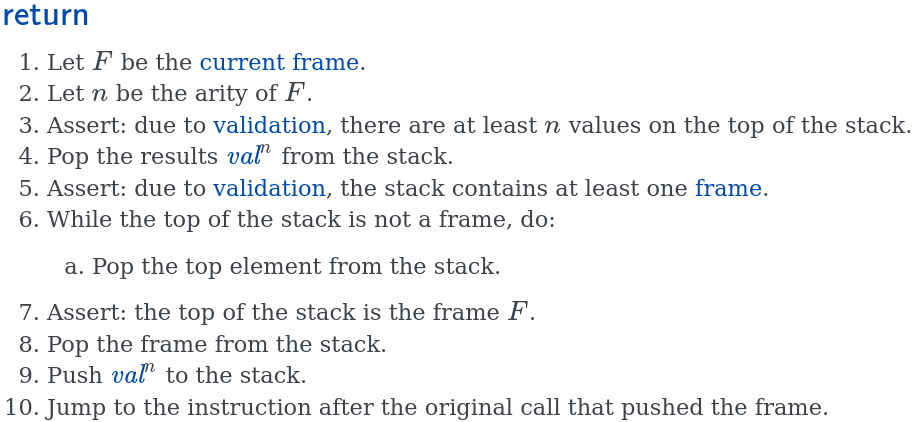
\includegraphics[height=0.8\textheight]{../sandbox/wasm-return-spec}
\end{frame}

\begin{frame}{WebAssembly as sandboxing}
    \begin{itemize}
    \item can compile existing C/C++ library using WebAssembly\ldots
    \item then call using language virtual machine
    \end{itemize}
\end{frame}



\section{sandboxing API: RLBox}
\begin{frame}{RLBox}
    \begin{itemize}
    \item saw interfaces for using sandboxes from user perspective?
    \item what about for privilege separation?
        \begin{itemize}
        \item recall: like Chrome separate renderer process idea
        \item need to navigate OS sandboxing API + create interface for sandboxed part?
        \end{itemize}
    \vspace{.5cm}
    \item some reusable tools have appeared for this (but no clear winner)
    \item one example: RLBox (published in Usenix Security 2020)
        \begin{itemize}
        \item Shravan Narayan and Craig Disselkoen, UC San Diego; Tal Garfinkel, Stanford University; Nathan Froyd and Eric Rahm, Mozilla; Sorin Lerner, UC San Diego; Hovav Shacham, UT Austin; Deian Stefan, UC San Diego
        \end{itemize}
    \end{itemize}
\end{frame}

\begin{frame}[fragile,label=rlboxusage]{RLBox usage}
\begin{itemize}
\item part of example from author's presentation:
    \begin{itemize}
    \item goal: invoke JPEG parser in sandbox
    \end{itemize}
\end{itemize}
\begin{lstlisting}[language=C++,style=script]
autosandbox = rlbox::create_sandbox<wasm>();
tainted<jpeg_decompress_struct*> p_jpeg_img = sandbox.malloc_in_sandbox<jpeg_decompress_struct>();
tainted<jpeg_source_mgr*> p_jpeg_input_source_mgr = sandbox.malloc_in_sandbox<jpeg_source_mgr>();
sandbox.invoke(jpeg_create_decompress, p_jpeg_img);
p_jpeg_img->src = p_jpeg_input_source_mgr;
p_jpeg_img->src->fill_input_buffer = ...;
sandbox.invoke(jpeg_read_header,p_jpeg_img/*...*/);
\end{lstlisting}
\begin{itemize}
\item tool handles running `jpeg\_create\_decompress', `jpeg\_read\_header' in sandbox
\item values shared with sandbox marked as ``tainted''
    \begin{itemize}
    \item C++ (template) class
    \end{itemize}
\item this example: using WebAssembly-based sandbox
\item used in firefox
\end{itemize}
\end{frame}


\section{application permissions}
\usetikzlibrary{calc}
\begin{frame}{some Android prompts}
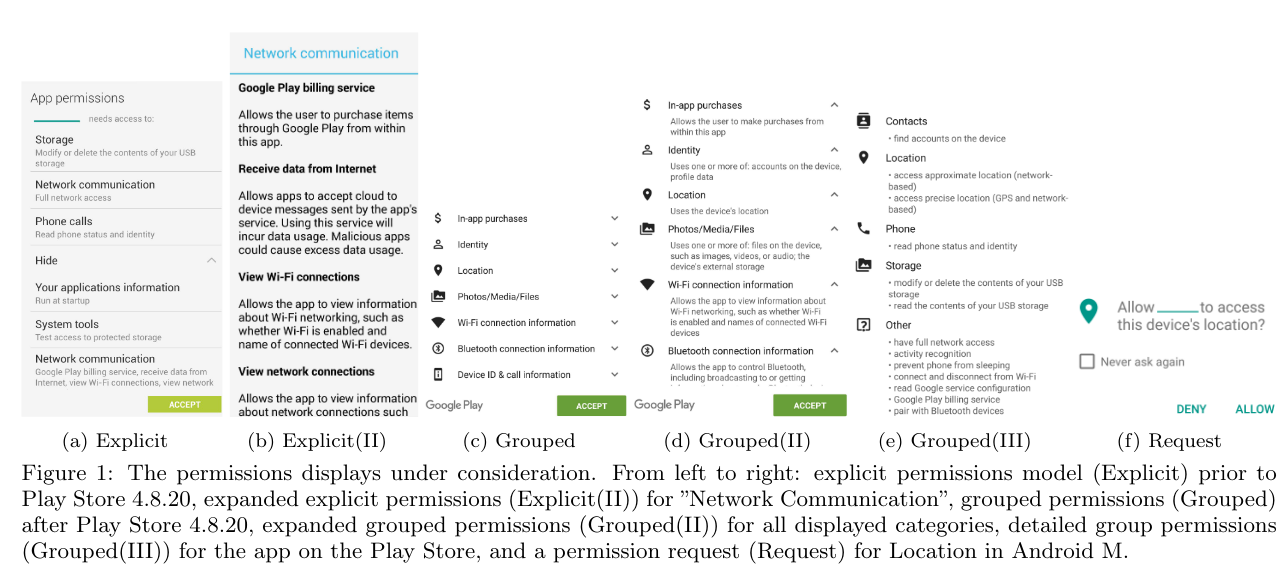
\includegraphics[width=\textwidth]{../sandbox/android-perm-screens}
\imagecredit{from Clark et al, ``No Time At All: Opportunity Cost of Android Permissions'' (HotWireless'16)}
\end{frame}


\subsection{UI problems}

\begin{frame}<1>[label=appPermUI]{UI problems with application permissions}
    \begin{itemize}
    \item \myemph<2>{do applications request sensible permissions?}
    \item \myemph<3>{do users pay attention to permission requests?}
    \item \myemph<3>{do users understand what permissions mean?}
    \item are permissions fine-grained enough?
    \item are permissions coarse-grained enough?
    \end{itemize}
\end{frame}


\subsection{do request right permissions?}
\againframe<2>{appPermUI}
\begin{frame}{right permissions?}
    \begin{itemize}
    \item Felt, Chin, Hanna, Song and Wagner, ``Android Permissions Demystified'' (CCS 2011)
    \item used static analysis to compare requested permissions to what applications did
        \begin{itemize}
        \item at the time: permissions requested at installation
        \end{itemize}
    \item sample of 900 applications
    \item estimate approx 200 over-privileged
        \begin{itemize}
        \item (estimate because using false positive rate from manual checking)
        \end{itemize}
    \end{itemize}
\end{frame}

\begin{frame}{why extra permissions?}
    \begin{itemize}
    \item selected from Felt et al's analysis:
    \item developers confused similar permissions
        \begin{itemize}
        \item \texttt{ACCESS\_NETWORK\_STATE} versus \texttt{ACCESS\_WIFI\_STATE}
        \end{itemize}
    \item developers thought permissions were needed for delegated tasks
        \begin{itemize}
        \item \texttt{CALL\_PHONE} not needed to invoke phone app
        \item \texttt{INSTALL\_APPLICATION} not needed to open app store install dialog
        \end{itemize}
    \item developers thought permissions needed for all methods of class
        \begin{itemize}
        \item \texttt{WRITE\_SETTINGS} when using (no-permission) read-settings operations
        \end{itemize}
    \item copy-and-paste
    \end{itemize}
\end{frame}


\subsection{do users understand permissions?}
\againframe<3>{appPermUI}
\begin{frame}{a user study (2012)}
    \begin{itemize}
    \item Felt, Ha, Egelman, Haney, Chin, Wagner, ``Android Permissions: User Attention, Comprehension, and Behavior''
    \item performed lab study; task: find + install coupon app
    \item at the time: Android prompted for permissions on installation
    \vspace{.5cm}
    \item<2-> 17\% looked at app permissions detail
    \item<2-> 42\% aware of permissions
    \item<2-> 42\% unaware of permissions
    \vspace{.5cm}
    \item<2-> versus: 88\% read reviews 
    \end{itemize}
\end{frame}

\begin{frame}{a user survey (2012)}
    \begin{itemize}
    \item same paper did survey about what permissions meant
    \item three multiple choice questions 
        \begin{itemize}
        \item selected from bank of 11
        \end{itemize}
    \item 302 respondents; 3 fully correct
    \item average 21\%
    \end{itemize}
\end{frame}

\begin{frame}{example survey question}
    \begin{itemize}
    \item `Read phone state and identity' allows which of these?
    \vspace{.5cm}
    \item Read your phone number
    \item See who you have called
    \item Track you across applications
    \item Load adverisements
    \end{itemize}
\end{frame}

\begin{frame}{survey questions (1)}
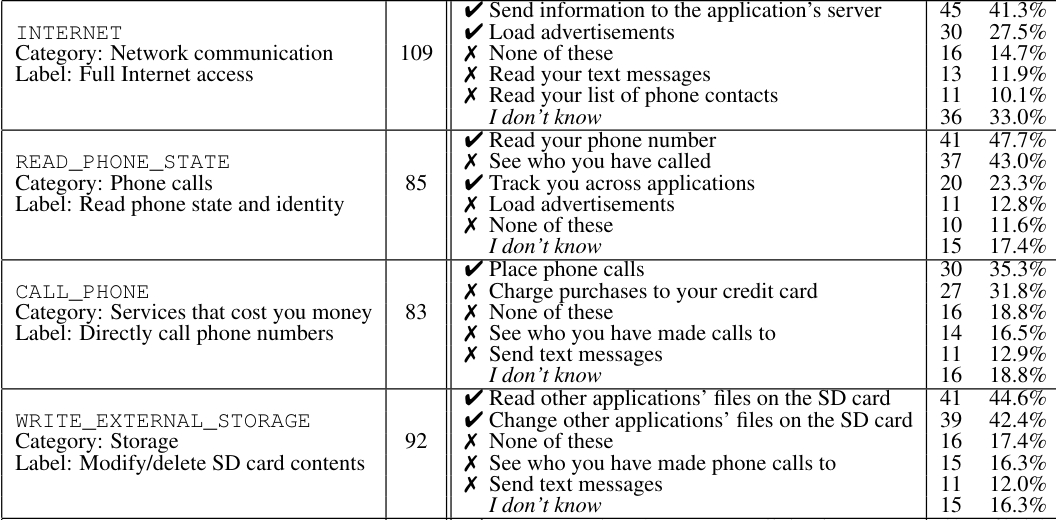
\includegraphics[width=\textwidth]{../sandbox/android-perm-survey1}
\end{frame}

\begin{frame}{survey questions (2)}
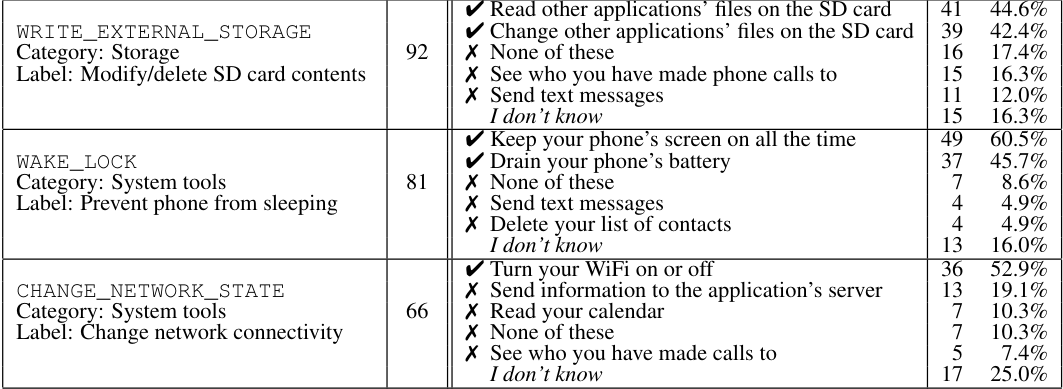
\includegraphics[width=\textwidth]{../sandbox/android-perm-survey2}
\end{frame}

\begin{frame}{survey questions (3)}
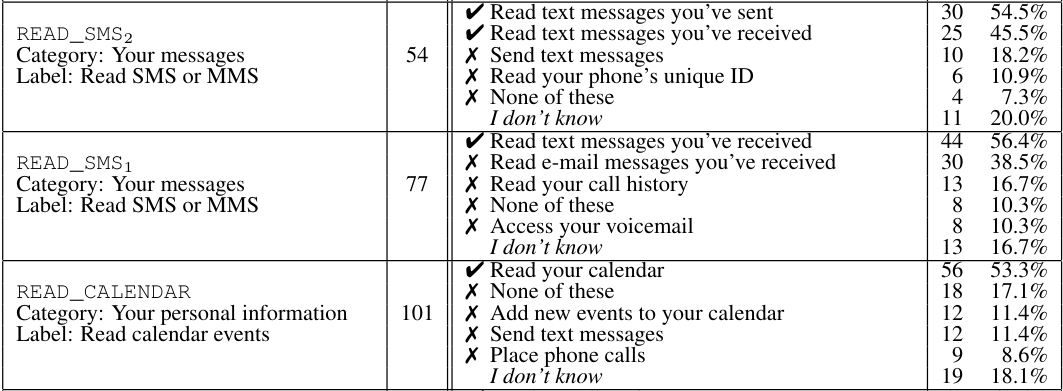
\includegraphics[width=\textwidth]{../sandbox/android-perm-survey3}
\end{frame}

\begin{frame}{survey questions (4)}
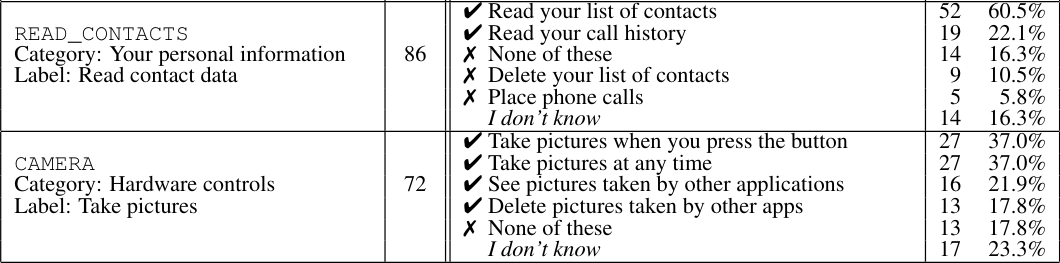
\includegraphics[width=\textwidth]{../sandbox/android-perm-survey4}
\end{frame}


\subsection{how to ask for permission?}
\begin{frame}
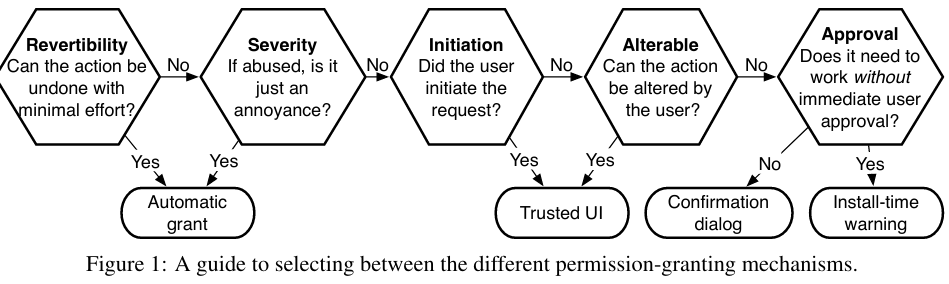
\includegraphics[width=\textwidth]{../sandbox/app-perm-how}
\scriptsize from Felt et al, ``How To Ask For Permission'' (HotSec'12)
\end{frame}

\begin{frame}{principles}
    \begin{itemize}
    \item Felt et al list ``principles'':
    \vspace{.5cm}
    \item ``Conserve user attention, utilizaing it for only permissions that have severe consquences''
        \begin{itemize}
        \item too many security warnings means users won't pay attention
        \end{itemize}
    \item ``When possible, avoid interrupting the user's primary task with explicit security decisions''
        \begin{itemize}
        \item users will dismiss warnings because they get in the way of work
        \end{itemize}
    \end{itemize}
\end{frame}


\subsection{permissions abuse: Cloak and Dagger}
\begin{frame}{Cloak and Dagger}

\includegraphics[width=\textwidth]{../sandbox/cloak-and-dagger}
\end{frame}

\begin{frame}{cloak and dagger permissions}
    \begin{itemize}
    \item the two permissions:
        \begin{itemize}
        \item SYSTEM\_ALERT\_WINDOW: \\
            draw windows on top of screen \\
            (at time: enabled by default)
        \item BIND\_ACCESSIBILITY\_SERVICE: \\
            ``Observe your actions'' \\
            ``Retrieve window content''
        \end{itemize}
    \item can hide window content while user interacts with it
    \item \ldots and stealthy get user to do more things
    \end{itemize}
\end{frame}

\begin{frame}{also, a clickjacking attack}
    \begin{itemize}
    \item at the time, could draw overlay window over permissions dialog
    \item \ldots convince user to press where ``OK'' button is
    \item countermeasure: permissions dialog would detect this, ignore clicks
    \vspace{.5cm}
    \item problem: wouldn't detect if overlay didn't cover enough of button
    \end{itemize}
\end{frame}


\subsection{permissions abuse: information leak}
\begin{frame}{privacy and permissions}
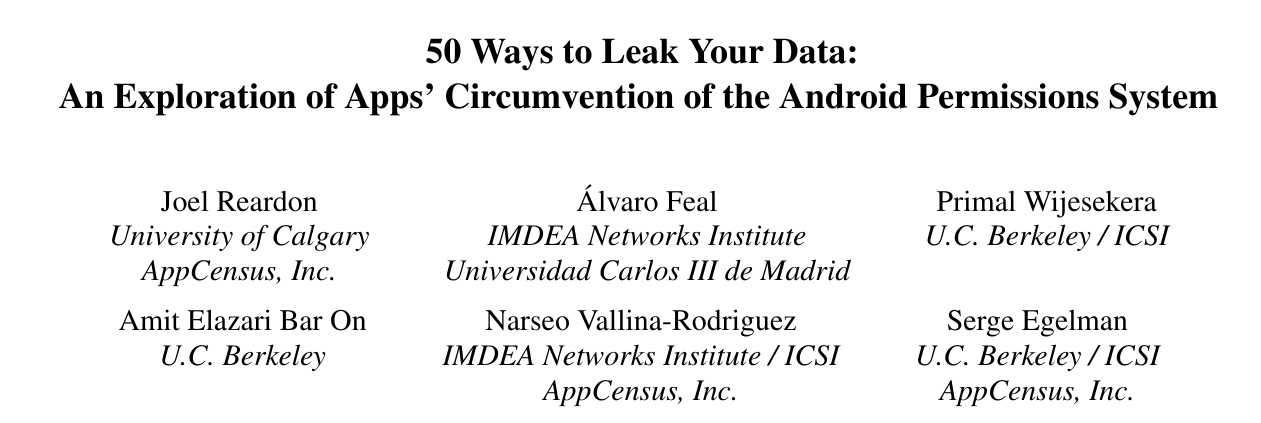
\includegraphics[width=0.7\textwidth]{../sandbox/priv-and-perm}
    \begin{itemize}
    \item 2019 paper
    \item many mobile application permissions related to privacy
    \item getting phone ID, email address, location, \ldots
    \item but applications (especially ad libraries) find workarounds
    \end{itemize}
\end{frame}

\begin{frame}{permissions being insufficient}
    \begin{itemize}
    \item permissions check limited API calls for getting private info,\ldots
    \item \ldots but there were alternative, unfiltered system calls for
    \vspace{.5cm}
    \item getting MAC address (effectively phone ID)
        \begin{itemize}
        \item Linux \texttt{ioctl} system call on socket
        \end{itemize}
    \item WiFi base station address
        \begin{itemize}
        \item ARP cache (recently seen machines on network, to know where to send packets)
        \end{itemize}
    \item location
        \begin{itemize}
        \item geolocation tag on recent photos
        \end{itemize}
    \end{itemize}
\end{frame}

\begin{frame}{covert channels}
    \begin{itemize}
    \item advertising libraries would store phone ID/account info in a file
        \begin{itemize}
        \item \ldots when they had permissions to retrieve it
        \end{itemize}
    \item and would read phone ID/account info from a file
        \begin{itemize}
        \item \ldots when they did not
        \end{itemize}
    \end{itemize}
\end{frame}


% FIXME: sandboxing and UIs


% FIXME: https://www.usenix.org/system/files/sec19-reardon.pdf
% FIXME: SFI and/or WAsm


\section{backup slides}
\begin{frame}{backup slides}
\end{frame}
